\section{最大延拓}
\label{sec:odeex-maximal}

Picard--Lindelöf定理只保证一小段时间。到达时间窗的尽头后，把终点当作新的初值再解一段，解就能接着往前走。这个过程能继续多久，走不下去时发生了什么？本节在定义~\ref{def:odeex-local-lipschitz}的条件下回答。以下总设$\bm{D}\subseteq\mathbb{R}\times\mathbb{R}^{n}$开，$\bm{f}:\bm{D}\to\mathbb{R}^{n}$连续，并在状态方向局部Lipschitz连续，该性质对时间局部一致。

\paragraph{相容的局部解}
拼接之前要确认，两段局部解在重叠处不会打架。局部唯一性只在一个小窗内成立，下面的引理把它传播到任意长的公共区间上，办法是看两条解重合的时刻组成的集合。

\begin{lemma}[公共区间上的唯一性]
\label{lem:odeex-common-uniqueness}
设$\bm{x}_1,\bm{x}_2$分别是区间$I_1,I_2$上的经典解，$I_1\cap I_2$含$t_0$，且$\bm{x}_1(t_0)=\bm{x}_2(t_0)$。则$\bm{x}_1=\bm{x}_2$在$I_1\cap I_2$上成立。
\end{lemma}

\begin{proof}
记$I=I_1\cap I_2$，它是区间。令$S=\{t\in I:\bm{x}_1(t)=\bm{x}_2(t)\}$，它含$t_0$。两条解连续，所以$S$在$I$中闭。

下面证明$S$在$I$中开。任取$t^\ast\in S$，记$\bm{x}^\ast=\bm{x}_1(t^\ast)$。在$(t^\ast,\bm{x}^\ast)$的邻域内，由定义~\ref{def:odeex-local-lipschitz}，可以取一个盒子和常数$M,L$，使定理~\ref{thm:odeex-picard-lindelof}的条件成立，得到时间窗$[t^\ast-\delta,t^\ast+\delta]$。

$\bm{x}_1,\bm{x}_2$在区间$I\cap[t^\ast-\delta,t^\ast+\delta]$上都是以$(t^\ast,\bm{x}^\ast)$为初值的经典解，由定理的结论2，它们都等于窗上的唯一解，所以这段区间包含在$S$中。

$I$是连通的，$S$是它的非空开闭子集，于是$S=I$。
\end{proof}

图~\ref{fig:odeex-gluing}(a)画的是两段解的重叠，引理保证重叠部分是同一条曲线。图(b)是证明的核心：若两条解有“第一次分开”的时刻$t^\ast$，在该时刻的状态附近局部唯一性就被破坏了，所以这样的时刻不存在。

\begin{BookInlineFigure}
  \centering
  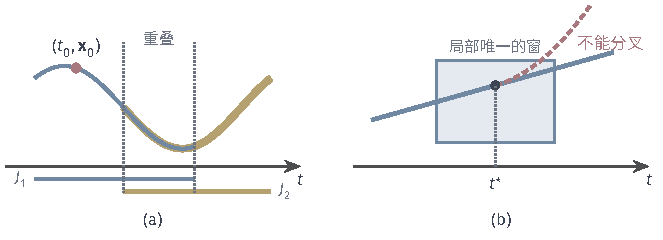
\includegraphics[width=112mm]{figures/06-differential-equations/01-ordinary-differential-equations/tikz/odeex-gluing/figure.pdf}
  \caption{局部解的相容性。(a)区间$J_1$（蓝）与$J_2$（黄）上的两段解经过同一初值，在重叠的时间段内是同一条曲线，并起来是更长区间上的解。(b)若两条解在$t^\ast$之后分开（红色虚线），在$(t^\ast,\bm{x}(t^\ast))$的小窗（浅蓝矩形）内就有两个解，与局部唯一性矛盾。}
  \label{fig:odeex-gluing}
\end{BookInlineFigure}

\paragraph{最大解}
有了相容性，就可以把所有局部解并起来。设$\bm{x}$是区间$I$上的解，$\tilde{\bm{x}}$是区间$\tilde I\supsetneq I$上的解，且$\tilde{\bm{x}}$在$I$上等于$\bm{x}$，就称$\tilde{\bm{x}}$是$\bm{x}$的一个\term{解的延拓}（continuation of a solution）。不能再延拓的解称为\term{最大解}（maximal solution），它的定义区间称为\term{最大存在区间}（maximal interval of existence）。

\begin{theorem}[最大解]
\label{thm:odeex-maximal}
对每点$(t_0,\bm{x}_0)\in\bm{D}$，初值问题~\eqref{eq:odeex-ivp}存在唯一的最大解$\bm{x}:I_{\max}\to\mathbb{R}^{n}$，其中$I_{\max}=(\omega_-,\omega_+)$是含$t_0$的开区间，$-\infty\leq\omega_-<\omega_+\leq+\infty$。该初值问题的每个解都是最大解在某个子区间上的限制。
\end{theorem}

\begin{proof}
设$\{(I_\alpha,\bm{x}_\alpha)\}$是该初值问题的全部解，由定理~\ref{thm:odeex-picard-lindelof}，这个族非空。各$I_\alpha$都含$t_0$，所以$I_{\max}=\bigcup_\alpha I_\alpha$是区间。对$t\in I_{\max}$，取含$t$的$I_\alpha$，令$\bm{x}(t)=\bm{x}_\alpha(t)$，由引理~\ref{lem:odeex-common-uniqueness}，这个值与$\alpha$的选取无关。

$t_0$到$t$的闭区间含于$I_\alpha$，在其上$\bm{x}=\bm{x}_\alpha$，所以$\bm{x}$在$t$处满足积分方程~\eqref{eq:odeex-integral}。这对每个$t\in I_{\max}$成立，且被积函数连续，因此$\bm{x}$是$I_{\max}$上的经典解。

$\bm{x}$不能延拓，否则延拓后的解属于上述族，其定义区间含于$I_{\max}$。每个解都是$\bm{x}$的限制，这由构造得到，唯一性随之成立。

最后证明$I_{\max}$是开区间。若右端点$\omega_+$属于$I_{\max}$，则$(\omega_+,\bm{x}(\omega_+))\in\bm{D}$，从这一点解局部初值问题，得到$[\omega_+-\delta,\omega_++\delta]$上的解$\bm{z}$。由引理~\ref{lem:odeex-common-uniqueness}，$\bm{z}$在左半段与$\bm{x}$相同。

令曲线在$I_{\max}$上等于$\bm{x}$、在$[\omega_+,\omega_++\delta]$上等于$\bm{z}$，它在$\omega_+$处连续，并在整个区间上满足积分方程，是比$\bm{x}$更长的解，矛盾。左端点同理。
\end{proof}

\paragraph{窗口为什么会越来越短}
以$\dot x=x^2$，$x(0)=1$为例，$\bm{D}=\mathbb{R}^{2}$，最大解是$1/(1-t)$，$I_{\max}=(-\infty,1)$。把“重启”过程具体算一遍，看看解为什么过不了$t=1$。

设已走到$(t_k,x_k)$，取半径$b=x_k$的盒子，$a$取得足够大，此时状态范围是$[0,2x_k]$，$M=4x_k^2$，第~\ref{sec:odeex-uniqueness}节的时间窗$\delta'=\min\{a,b/M\}$给出
\[
 \delta_k=\frac{x_k}{4x_k^2}=\frac{1}{4x_k}=\frac{1-t_k}{4}.
\]
最后一步用了$x_k=1/(1-t_k)$。于是下一个重启时刻满足$1-t_{k+1}=\tfrac34(1-t_k)$，从$t_0=0$开始，
\[
 t_k=1-\Bigl(\frac34\Bigr)^{k},\qquad x_k=\Bigl(\frac43\Bigr)^{k},\qquad\delta_k=\frac14\Bigl(\frac34\Bigr)^{k}.
\]

前几个重启时刻是
\[
 t_1=0.25,\quad t_2=0.4375,\quad t_3\approx0.5781.
\]
窗口长度成等比下降，总和恰好是$1$，无限次重启也越不过$t=1$，如图~\ref{fig:odeex-continuation-windows}。窗口变短的原因是状态增大，箭头变快，同样高度的盒子能撑的时间变短。

\begin{BookInlineFigure}
  \centering
  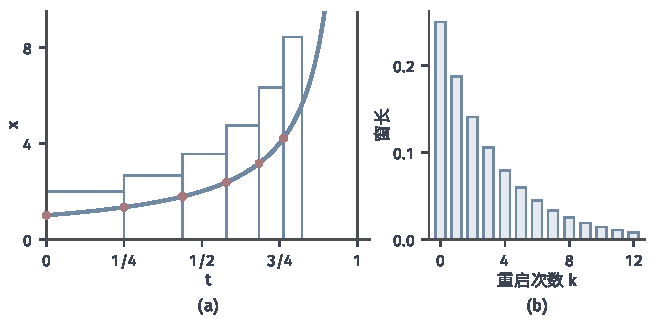
\includegraphics[width=112mm]{figures/06-differential-equations/01-ordinary-differential-equations/matplotlib/odeex-continuation-windows/figure.pdf}
  \caption{沿$\dot x=x^2$重启局部定理。(a)蓝线是真解，红点是重启点$(t_k,x_k)$，矩形是每次重启所用的时间窗$\delta_k$与状态范围$[0,2x_k]$，灰色竖线是$t=1$。(b)窗长$\delta_k=\tfrac14(3/4)^k$随重启次数按等比衰减，总和为$1$。}
  \label{fig:odeex-continuation-windows}
\end{BookInlineFigure}

这个例子提示了一般规律。时间窗只依赖盒子内的$M$和$L$。如果解始终留在一个固定的紧集内，$M,L$有共同的上界，窗口有一个不随重启变化的正下限，重启有限次就能越过任何有限时刻。所以解走不下去，只能是因为它没有留在任何紧集内。

\paragraph{紧集上的统一时间窗}
把这个想法写严格，需要两个引理：局部Lipschitz常数在紧集上可以取成统一的，局部定理的时间窗在紧集上也可以取成统一的。

\begin{lemma}[紧集上的统一Lipschitz常数]
\label{lem:odeex-compact-lipschitz}
设$\bm{K}\subseteq\bm{D}$是紧集。则存在常数$L$，使式~\eqref{eq:odeex-lipschitz}对$\bm{K}$中所有同一时刻的两点$(t,\bm{x}),(t,\bm{y})$成立。
\end{lemma}

\begin{proof}
设$M=\max_{\bm{K}}\lVert\bm{f}\rVert_2$。假设结论不成立，则对每个正整数$j$，存在$\bm{K}$中同一时刻的两点$(t_j,\bm{x}_j),(t_j,\bm{y}_j)$，使
\[
 \lVert\bm{f}(t_j,\bm{x}_j)-\bm{f}(t_j,\bm{y}_j)\rVert_2>j\lVert\bm{x}_j-\bm{y}_j\rVert_2.
\]
左端不超过$2M$，所以$\lVert\bm{x}_j-\bm{y}_j\rVert_2<2M/j\to0$。

由紧性，取子列使$(t_j,\bm{x}_j)$收敛到某点$(t_\ast,\bm{x}_\ast)\in\bm{K}$，此时$(t_j,\bm{y}_j)$也收敛到同一点。该点有定义~\ref{def:odeex-local-lipschitz}中的邻域和常数$L_\ast$，当$j$足够大时两点都在这个邻域内，不等号的左端不超过$L_\ast\lVert\bm{x}_j-\bm{y}_j\rVert_2$，再取$j>L_\ast$即得矛盾。
\end{proof}

\begin{lemma}[紧集上的统一时间窗]
\label{lem:odeex-uniform-window}
设$\bm{K}\subseteq\bm{D}$是紧集。则存在$\delta_{\bm{K}}>0$，使对每点$(s,\bm{\xi})\in\bm{K}$，以$(s,\bm{\xi})$为初值的问题在$[s-\delta_{\bm{K}},s+\delta_{\bm{K}}]$上有解。
\end{lemma}

\begin{proof}
若$\bm{D}$不是全空间，紧集$\bm{K}$到闭集$\bm{D}^{\mathrm{c}}$的距离大于零，取正数$\rho$小于这个距离的一半，否则取$\rho=1$。令
\[
 \bm{K}'=\bigl\{(t,\bm{x}):\exists(s,\bm{\xi})\in\bm{K},\ \lvert t-s\rvert\leq\rho/2,\ \lVert\bm{x}-\bm{\xi}\rVert_2\leq\rho/2\bigr\}.
\]
$\bm{K}'$是$\bm{K}$与一个紧盒子的和，因而紧，并且$\bm{K}'\subseteq\bm{D}$。

在$\bm{K}'$上取$M>0$为$\lVert\bm{f}\rVert_2$的上界，由引理~\ref{lem:odeex-compact-lipschitz}取$L>0$。对$\bm{K}$中任一点，$a=b=\rho/2$的盒子都含于$\bm{K}'$，定理~\ref{thm:odeex-picard-lindelof}给出共同的时间窗
\[
 \delta_{\bm{K}}=\min\Bigl\{\frac{\rho}{2},\frac{\rho}{2M},\frac{1}{2L}\Bigr\}.
\]
这就是所要的常数。
\end{proof}

\paragraph{离开每个紧集}
现在可以把“走不下去”说清楚。

\begin{theorem}[最大解离开紧集]
\label{thm:odeex-escape}
设$\bm{x}:(\omega_-,\omega_+)\to\mathbb{R}^{n}$是最大解。对每个紧集$\bm{K}\subseteq\bm{D}$，存在$t_{\bm{K}}\in(\omega_-,\omega_+)$，使当$t\in(t_{\bm{K}},\omega_+)$时，都有$(t,\bm{x}(t))\notin\bm{K}$。左端点$\omega_-$有对称的结论。
\end{theorem}

\begin{proof}
反设存在紧集$\bm{K}$和$t_j\uparrow\omega_+$，使$(t_j,\bm{x}(t_j))\in\bm{K}$。$\bm{K}$在时间方向有界，所以$\omega_+<+\infty$。

取引理~\ref{lem:odeex-uniform-window}中的$\delta_{\bm{K}}$，再取$j$使$t_j+\delta_{\bm{K}}>\omega_+$。以$(t_j,\bm{x}(t_j))$为初值的解$\bm{z}$在$[t_j-\delta_{\bm{K}},t_j+\delta_{\bm{K}}]$上存在，由引理~\ref{lem:odeex-common-uniqueness}，它在公共区间上与$\bm{x}$相同。

$\bm{z}$的定义区间越过了$\omega_+$，把$\bm{x}$与$\bm{z}$并起来就得到比最大解更长的解，矛盾。
\end{proof}

注意结论是“最终离开并且不再回来”，比“离开过”强。证明正是靠这一点：只要解在$\omega_+$附近回到$\bm{K}$一次，时间窗就能把它带过$\omega_+$。

\paragraph{两种障碍}
最常见的定义域是乘积形式$\bm{D}=J\times\bm{\Omega}$，其中$J$是右端给定的开时间区间，$\bm{\Omega}\subseteq\mathbb{R}^{n}$是开集。设$\omega_+<\sup J$，即解在右端还有定义的时候就停止了。对$\bm{\Omega}$的每个紧子集$\bm{C}$，$[t_0,\omega_+]\times\bm{C}$是$\bm{D}$的紧子集，由定理~\ref{thm:odeex-escape}，$\bm{x}(t)$在$\omega_+$之前最终离开$\bm{C}$。

特别地，状态空间是整个$\mathbb{R}^{n}$时，取$\bm{C}$为半径任意大的闭球，得到：若$\omega_+<\sup J$，则
\begin{equation}
 \lim_{t\uparrow\omega_+}\lVert\bm{x}(t)\rVert_2=+\infty.
 \label{eq:odeex-blowup-alternative}
\end{equation}
这就是有限时间爆炸。对一般的$\bm{\Omega}$，紧子集可以取成“离$\bm{\Omega}$的边界不太近且范数不太大”的集合，解要离开它们，要么范数趋于无穷，要么趋近$\bm{\Omega}$的边界，也可能在两者之间来回。

图~\ref{fig:odeex-exit-obstacles}给出三种典型情况，三个方程的右端都在各自定义域内满足本节的条件，$\omega_+=1$。

\begin{BookInlineFigure}
  \centering
  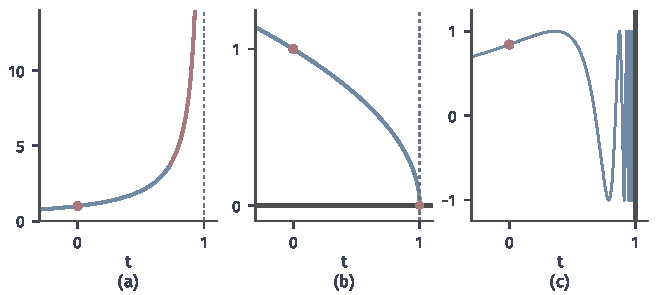
\includegraphics[width=112mm]{figures/06-differential-equations/01-ordinary-differential-equations/matplotlib/odeex-exit-obstacles/figure.pdf}
  \caption{最大解在$\omega_+=1$处结束的三种情形，红点是初值，灰色粗线是定义域的边界。(a)$\dot x=x^2$，$\bm{D}=\mathbb{R}^{2}$，状态趋于无穷（红色部分）。(b)$\dot x=-1/(2x)$，$\bm{D}=\mathbb{R}\times(0,\infty)$，解$\sqrt{1-t}$有界，趋近状态边界$x=0$。(c)$\bm{D}=(-\infty,1)\times\mathbb{R}$，解$\sin(1/(1-t))$有界且没有极限，时间到达定义域的边界$t=1$。}
  \label{fig:odeex-exit-obstacles}
\end{BookInlineFigure}

图(a)是状态无界的障碍：$\bm{\Omega}=\mathbb{R}$，解按式~\eqref{eq:odeex-blowup-alternative}趋于无穷。图(b)是逼近定义域边界的障碍：对$\dot x=-1/(2x)$，$x(0)=1$，由$(x^2)'=-1$得到$x=\sqrt{1-t}$，它在$t\uparrow1$时有界地趋于$0$，而$0$不在$\bm{\Omega}=(0,\infty)$中，右端在那里无定义，解不能再走。

图(c)是时间区间本身的端点：方程$\dot x=\cos\bigl(1/(1-t)\bigr)/(1-t)^2$，$x(0)=\sin1$的解是$\sin\bigl(1/(1-t)\bigr)$。此时$\omega_+=\sup J=1$，不属于式~\eqref{eq:odeex-blowup-alternative}的情形，定理~\ref{thm:odeex-escape}仍然成立，因为$(t,\bm{x}(t))$的时间分量趋向$\bm{D}$的边界。解有界但在$t\uparrow1$时没有极限，可见“离开紧集”不等于“收敛到某个边界点”。
